%-------------------------------------------------------------------------------
% CAPITOLO 19
%-------------------------------------------------------------------------------
\chapter{Lezione 19}
\label{capitolo_19}

\section{Funzione di Correlazione}
Iniziamo definendo la funzione di correlazione connessa $C_{ij}^c$ tra due spin $S_i$ e $S_j$ situati nei siti $i$ e $j$ di un reticolo:

\begin{equation} \label{eq:ch19_1}
C_{ij}^{c} = \langle S_i S_j \rangle - \langle S_i \rangle \langle S_j \rangle
\end{equation}

Nell'approssimazione di campo medio, che considera il miglior modello non interattivo per approssimare il nostro modello fortemente interattivo, le funzioni di correlazione risultano essere zero. Questo avviene perché, intrinsecamente, tale approssimazione annulla le correlazioni, anche se nel sistema reale (senza approssimazione) esse non sono nulle.
Per calcolare comunque queste funzioni di correlazione nel contesto in cui stiamo lavorando, possiamo sfruttare il Teorema Fluttuazione-Dissipazione (FDT). Questo teorema mette in relazione la funzione di correlazione magnetica con la suscettibilità del sistema. La relazione è la seguente:

\begin{equation} \label{eq:ch19_2}
\chi_{ij} = \beta C_{ij}^{c}
\end{equation}

dove $\chi_{ij}$ è la matrice di suscettibilità, definita come la funzione di risposta che descrive la risposta lineare del sistema all'applicazione di un campo esterno $h_j$:

\begin{equation} \label{eq:ch19_3}
\chi_{ij} = \frac{\partial \langle S_i \rangle}{\partial h_j} \bigg|_{h=0}
\end{equation}

Possiamo calcolare la funzione di suscettibilità nell'approssimazione di campo medio. Quindi, attraverso la FDT, otteniamo in modo indiretto la funzione di correlazione stessa.


\section{Invarianza Traslazionale e Spazio di Fourier}
Le funzioni $C_{ij}$ e $\chi_{ij}$ dipendono dalle posizioni spaziali dei siti $i$ e $j$, che indichiamo con $\bar{r}_i$ e $\bar{r}_j$.
Consideriamo un sistema definito su un reticolo regolare, ad esempio un reticolo 2D dove ogni spin $S_i$ è localizzato in una specifica posizione $\bar{r}_i$.
In assenza di un campo magnetico esterno, il sistema è perfettamente invariante per traslazioni spaziali. Di conseguenza, una funzione che in principio dipende da due coordinate $\bar{r}_i$ e $\bar{r}_j$, come $C^c(\bar{r}_i, \bar{r}_j)$, dipenderà in realtà solo dalla loro distanza relativa $\bar{r}_{ij} = \bar{r}_i - \bar{r}_j$:

\begin{equation} \label{eq:ch19_4}
C^c(\bar{r}_i, \bar{r}_j) \rightarrow C^c(\bar{r}_{ij})
\end{equation}

Lo stesso vale per la suscettibilità:

\begin{equation} \label{eq:ch19_5}
\chi(\bar{r}_i, \bar{r}_j) \rightarrow \chi(\bar{r}_{ij})
\end{equation}

Questo significa che il comportamento fisico tra due punti $i$ e $j$ non dipende specificamente dalla loro posizione assoluta nel reticolo, ma solo dalla loro distanza relativa (assumendo condizioni al contorno periodiche o di essere lontani dai bordi).
Se il modello possiede anche invarianza rotazionale (isotropia), allora la dipendenza sarà solo dal modulo della distanza, $r_{ij} = |\bar{r}_{ij}|$.
L'invarianza traslazionale rende conveniente lavorare nello spazio di Fourier. La trasformata di Fourier di una funzione dipendente solo da $\bar{r}_{ij}$ dipenderà da un solo vettore d'onda $\bar{q}$.
Per la funzione di correlazione connessa e la suscettibilità avremo:

\begin{equation} \label{eq:ch19_6}
C^c(\bar{r}_{ij}) \xrightarrow{\text{Fourier T.}} \hat{C}^c(\bar{q})
\end{equation}

\begin{equation} \label{eq:ch19_7}
\chi(\bar{r}_{ij}) \xrightarrow{\text{Fourier T.}} \hat{\chi}(\bar{q}) = \frac{\partial \hat{m}(\bar{q})}{\partial \hat{h}(\bar{q})}
\end{equation}

dove $\hat{m}(\bar{q})$ e $\hat{h}(\bar{q})$ sono le trasformate di Fourier della magnetizzazione e del campo magnetico, rispettivamente. La strategia consiste nel calcolare $\hat{\chi}(\bar{q})$, da cui si ottiene $\hat{C}^c(\bar{q})$ tramite la FDT, e infine antitrasformando per ottenere $C^c(\bar{r}_{ij})$.
Il punto di partenza è l'equazione di campo medio per la magnetizzazione $m_i$ sul sito $i$. Nel caso di un campo omogeneo $h$, tutte le magnetizzazioni locali $m_i$ sono uguali alla magnetizzazione globale $m$, e l'equazione è:

\begin{equation} \label{eq:ch19_8}
m = \tanh(\beta h + \beta J z m)
\end{equation}

dove $z$ è il numero di primi vicini e $J$ è la costante di accoppiamento.
Per calcolare la suscettibilità $\chi_{ij}$, che descrive la risposta a un campo locale $h_j$, dobbiamo generalizzare l'equazione di campo medio al caso in cui il campo $h_i$ può variare da sito a sito (campo disomogeneo). In questo caso, anche la magnetizzazione media locale $m_i = \langle S_i \rangle$ varierà da sito a sito. L'equazione generalizzata diventa:

\vspace{0.5cm}
\noindent\fbox{%
    \parbox{\dimexpr\linewidth-2\fboxsep-2\fboxrule\relax}{%
        \begin{equation} \label{eq:ch19_9}
        m_i = \tanh\left(\beta h_i + \beta J \sum_{l \in N_i} m_l\right)
        \end{equation}
    }%
}
\vspace{0.5cm}

dove $N_i$ indica l'insieme dei primi vicini del sito $i$.
Risolvere questo sistema di $N$ equazioni accoppiate per $m_i$ nello spazio reale è complicato perché non è direttamente invertibile. Per questo motivo, passiamo allo spazio di Fourier, dove le equazioni si disaccoppiano e diventano invertibili.


\section{Linearizzazione e Trasformata di Fourier}
Vogliamo studiare il comportamento della suscettibilità e della funzione di correlazione vicino alla temperatura critica $T_c$, approcciandola dalla fase ad alta temperatura ($T \rightarrow T_c^+$). In questa regione, la magnetizzazione è zero in assenza di campo.
Se applichiamo un campo $h_i$ molto piccolo, anche la risposta $m_i$ sarà piccola. Possiamo quindi espandere la tangente iperbolica al primo ordine ($\tanh(x) \approx x$ per $x \ll 1$). L'equazione linearizzata diventa:

\begin{equation} \label{eq:ch19_10}
m_i \approx \beta h_i + \beta J \sum_{l \in N_i} m_l
\end{equation}

Definiamo la trasformata di Fourier discreta e la sua inversa come segue:

\begin{equation} \label{eq:ch19_11}
\hat{m}_{\bar{q}} = \sum_{\bar{r}_i} e^{-i\bar{q}\cdot\bar{r}_i} m_i
\end{equation}

\begin{equation} \label{eq:ch19_12}
m_i = \frac{1}{N} \sum_{\bar{q}} e^{i\bar{q}\cdot\bar{r}_i} \hat{m}_{\bar{q}}
\end{equation}

La posizione del fattore $1/N$ è convenzionale.
Applichiamo la trasformata di Fourier all'equazione linearizzata:
\begin{itemize}
    \item Il membro sinistro $m_i$ diventa $\hat{m}_{\bar{q}}$
    \item Il termine $\beta h_i$ diventa $\beta \hat{h}_{\bar{q}}$
\end{itemize}

Per il termine di interazione, dobbiamo essere più attenti:

\begin{equation} \label{eq:ch19_13}
\text{TF}\left[\beta J \sum_{j \in N_i} m_j\right] = \sum_{\bar{r}_i} e^{-i\bar{q}\cdot\bar{r}_i} \beta J \sum_{l \in N_i} \left(\frac{1}{N} \sum_{\bar{k}} e^{i\bar{k}\cdot\bar{r}_l} \hat{m}_{\bar{k}}\right)
\end{equation}

Ponendo $\bar{r}_l = \bar{r}_i + \bar{r}_{il}$:

\begin{equation} \label{eq:ch19_14}
\frac{\beta J}{N} \sum_{\bar{r}_i} e^{-i\bar{q}\cdot\bar{r}_i} \sum_{l \in N_i} \sum_{\bar{k}} e^{i\bar{k}\cdot(\bar{r}_i + \bar{r}_{il})} \hat{m}_{\bar{k}}
\end{equation}

Raggruppiamo i termini che dipendono da $\bar{r}_i$:

\begin{equation} \label{eq:ch19_15}
\frac{\beta J}{N} \sum_{\bar{k}} \sum_{\bar{r}_i} e^{-i\bar{r}_i \cdot (\bar{q}-\bar{k})} \left( \sum_{l \in N_i} e^{i\bar{k}\cdot\bar{r}_{il}} \right) \hat{m}_{\bar{k}}
\end{equation}

La somma $\frac{1}{N}\sum_{\bar{r}_i} e^{-i(\bar{q}-\bar{k})\cdot\bar{r}_i}$ è una rappresentazione della delta di Kronecker $\delta(\bar{q}-\bar{k})$, quindi:

\begin{equation} \label{eq:ch19_16}
\beta J \sum_{\bar{k}} \delta(\bar{q}-\bar{k}) \left( \sum_{l \in N_i} e^{i\bar{k}\cdot\bar{r}_{il}} \right) \hat{m}_{\bar{k}}
\end{equation}

La presenza della $\delta$ nella somma su $\bar{k}$ significa che solo il termine con $\bar{k}=\bar{q}$ sopravvive:

\begin{equation} \label{eq:ch19_17}
\beta J  \left( \sum_{l \in N_i} e^{i\bar{q}\cdot\bar{r}_{il}} \right) \hat{m}_{\bar{q}}
\end{equation}

La somma $\sum_{l \in N_i} e^{i\bar{q}\cdot\bar{r}_{il}}$ è una somma sui vettori che connettono il sito $i$ ai suoi primi vicini. Per un reticolo regolare, questa somma ha lo stesso valore per ogni sito $i$ e non dipende da $\bar{r}_i$.
Per un reticolo ipercubico $d$-dimensionale con passo reticolare $L$, i vettori $\bar{r}_{il}$ che connettono ai primi vicini sono $(\pm L, 0, \dots)$, $(0, \pm L, \dots)$, ecc. La somma diventa:

\begin{equation} \label{eq:ch19_18}
\sum_{l \in N_i} e^{i\bar{q}\cdot\bar{r}_{il}} = \sum_{\alpha=1}^{d} (e^{iq_{\alpha}L} + e^{-iq_{\alpha}L}) = \sum_{\alpha=1}^{d} 2\cos(q_{\alpha}L)
\end{equation}

L'equazione trasformata completa è quindi:

\begin{equation} \label{eq:ch19_19}
\hat{m}_{\bar{q}} = \beta \hat{h}_{\bar{q}} + \beta J \hat{m}_{\bar{q}} \sum_{\alpha=1}^{d} 2\cos(q_{\alpha}L)
\end{equation}

Risolvendo per $\hat{m}_{\bar{q}}$:

\begin{equation} \label{eq:ch19_20}
\hat{m}_{\bar{q}} = \frac{\beta \hat{h}_{\bar{q}}}{1 - 2\beta J \sum_{\alpha=1}^{d} \cos(q_{\alpha}L)}
\end{equation}

Dalla definizione $\hat{\chi}(\bar{q}) =\frac{\partial \hat{m}_{\bar{q}} }{ \partial \hat{h}_{\bar{q}}}$, e usando $\hat{C}^c(\bar{q}) = \frac{1}{\beta} \hat{\chi}(\bar{q})$, otteniamo:

\begin{equation} \label{eq:ch19_21}
\hat{C}^c(\bar{q}) = \frac{1}{1 - 2\beta J \sum_{\alpha=1}^{d} \cos(q_{\alpha}L)}
\end{equation}

Siamo interessati al comportamento della funzione di correlazione a grandi distanze nello spazio reale: $r \gg L$. Questo corrisponde a piccoli vettori d'onda nello spazio di Fourier: $qL \ll 1$.
In questo limite, possiamo espandere il coseno: $\cos(x) \approx 1 - x^2/2$
Il denominatore di $\hat{C}^c(\bar{q})$ diventa:

\begin{align*}
1 - 2\beta J \sum_{\alpha=1}^{d} \cos(q_{\alpha}L) &\approx 1 - 2\beta J \sum_{\alpha=1}^{d} \left(1 - \frac{(q_{\alpha}L)^2}{2}\right) \\
&= 1 - 2\beta J d + \beta J L^2 \sum_{\alpha=1}^{d} q_{\alpha}^2 \\
&= 1 - \beta J z + \beta J L^2 q^2
\end{align*}

dove $z = 2d$ è il numero di coordinazione per un reticolo ipercubico e $q^2 = \sum_{\alpha} q_{\alpha}^2$ è il modulo quadro del vettore d'onda.
Quindi, per $q \ll 1/L$:

\begin{equation} \label{eq:ch19_22}
\hat{C}^c(\bar{q}) \approx \frac{1}{1 - \beta J z + \beta J L^2 q^2} = \frac{1}{\beta J L^2} \frac{1}{q^2 + \frac{1-\beta J z}{\beta J L^2}}
\end{equation}

Definiamo la lunghezza di correlazione $\xi$ come:

\vspace{0.5cm}
\noindent\fbox{%
    \parbox{\dimexpr\linewidth-2\fboxsep-2\fboxrule\relax}{%
        \begin{equation} \label{eq:ch19_23}
        \xi^{-2} = \frac{1 - \beta J z}{\beta J L^2}
        \end{equation}
    }%
}
\vspace{0.5cm}

Con questa definizione, $\hat{C}^c(\bar{q})$ assume la forma Ornstein-Zernike:

\vspace{0.5cm}
\noindent\fbox{%
    \parbox{\dimexpr\linewidth-2\fboxsep-2\fboxrule\relax}{%
        \begin{equation} \label{eq:ch19_24}
        \hat{C}^c(\bar{q}) = \frac{1}{\beta J L^2} \frac{1}{q^2 + \xi^{-2}}
        \end{equation}
    }%
}
\vspace{0.5cm}

La lunghezza di correlazione $\xi$ ha le dimensioni di una lunghezza. Ricordando che la temperatura critica di campo medio è $T_c = Jz/k_B$, ovvero $\beta_c J z = 1$, possiamo riscrivere $\xi$ come:

\begin{equation} \label{eq:ch19_25}
\xi = \sqrt{\frac{\beta J L^2}{1 - \beta J z}} = \frac{L \sqrt{\beta J}}{\sqrt{1 - \frac{T_c}{T}}}
\end{equation}


\section{Funzione di Correlazione nello Spazio Reale}
Per ottenere la funzione di correlazione nello spazio reale $C^c(\bar{r})$, dobbiamo antitrasformare.
Poiché siamo interessati a grandi distanze, possiamo passare a una trasformata di Fourier continua:

\begin{equation} \label{eq:ch19_26}
C^c(\bar{r}) = \int \frac{d^d q}{(2\pi)^d} e^{i\bar{q}\cdot\bar{r}} \hat{C}^c(\bar{q}) \approx A' \int d^d q \frac{e^{i\bar{q}\cdot\bar{r}}}{q^2 + \xi^{-2}}
\end{equation}

dove $A'$ è una costante.
Consideriamo il caso tridimensionale ($d=3$). L'integrale si calcola passando in coordinate sferiche per $\bar{q}$:

\begin{align} \label{eq:ch19_27}
C^c(\bar{r}) &= A \int_{-1}^{1} d(\cos\theta) \int_0^\infty dq \, q^2 \frac{e^{iqr\cos\theta}}{q^2 + \xi^{-2}} \nonumber \\ 
&=  A \int_0^\infty dq \, q^2 \frac{1}{iqr} \frac{[e^{iqr} - e^{-iqr}]}{q^2 + \xi^{-2}}  \nonumber \\ 
&= \frac{A}{ir} \int_0^\infty dq \frac{q}{q^2 + \xi^{-2}} [e^{iqr} - e^{-iqr}]
\end{align}

L'integrale da $0$ a $\infty$ viene esteso da $-\infty$ a $\infty$ (l'integrando completo è pari, quindi si introduce un fattore $1/2$ assorbito in $A$).
Si considera solo uno dei due termini esponenziali, $e^{iqr}$, poiché il calcolo per $e^{-iqr}$ è analogo e darà un contributo con segno opposto che si sommerà costruttivamente.

\begin{equation*}
\frac{A}{ir} \int_{-\infty}^\infty dq \frac{q e^{iqr}}{(q+i\xi^{-1})(q-i\xi^{-1})}
\end{equation*}

L'integrando ha due poli semplici nel piano complesso, in $q = i\xi^{-1}$ e $q = -i\xi^{-1}$.
Per il termine con $e^{iqr}$ ($r>0$), si chiude il contorno di integrazione nel semipiano superiore, includendo solo il polo $q = i\xi^{-1}$. L'integrale è pari a $2\pi i$ volte il residuo in questo polo.
Il residuo è $\frac{i\xi^{-1} e^{i(i\xi^{-1})r}}{2i\xi^{-1}} = \frac{1}{2}e^{-r/\xi}$.
Considerando entrambi i termini esponenziali, e tutti i fattori, si ottiene il risultato finale:

\begin{equation} \label{eq:ch19_28}
C^c(r) = A \frac{e^{-r/\xi}}{r}
\end{equation}

dove $A$ è un'altra costante e $r=|\bar{r}|$.
La funzione di correlazione decade esponenzialmente con la distanza, con una lunghezza $\xi$.

\textbf{Significato di $\xi$:}
La lunghezza di correlazione $\xi$ misura la scala di distanza su cui gli spin sono significativamente correlati.
\begin{itemize}
    \item \textbf{Alta temperatura ($T \gg T_c$):} Il rumore termico domina: $\beta J z = T_c/T \ll 1$. Quindi $\xi \approx L\sqrt{\beta J}$, che è piccola, dell'ordine della spaziatura reticolare $L$. Le correlazioni sono a corto raggio.
    \item \textbf{Avvicinandosi a $T_c$ (da $T > T_c$):} Il termine $(1 - T_c/T)$ al denominatore di $\xi$ diventa piccolo, quindi $\xi$ aumenta. Le fluttuazioni diventano correlate su distanze sempre maggiori.
    \item \textbf{Alla temperatura critica ($T = T_c$):} $\xi \rightarrow \infty$. La funzione di correlazione non decade più esponenzialmente, ma segue una legge di potenza. Per $d=3$, $e^{-r/\xi}/r \rightarrow 1/r$ per $\xi \rightarrow \infty$.
\end{itemize}

\begin{equation} \label{eq:ch19_29}
C^c(r) \xrightarrow{T=T_c} \frac{A}{r}
\end{equation}

Questo comportamento è detto scale-free (privo di scala), poiché non c'è una lunghezza caratteristica intrinseca nel decadimento. L'esponente con cui $\xi$ diverge vicino a $T_c$, $\xi \sim |T-T_c|^{-\nu}$, definisce un esponente critico $\nu$. Nel nostro caso di campo medio, $\nu = 1/2$.
In un sistema di dimensioni finite $L_{sys}$, la lunghezza di correlazione non può divergere all'infinito, ma sarà limitata da $L_{sys}$. Al punto critico, si trova che $\xi \sim L_{sys}$.


\section{Modello di Heisenberg e Rottura di Simmetria}
Il modello di Ising considera spin scalari ($S_i = \pm 1$). Una generalizzazione è il modello di Heisenberg, dove gli spin sono vettori $\bar{S}_i$ di norma fissata $|\bar{S}_i|=1$ che possono puntare in qualsiasi direzione nello spazio. L'Hamiltoniana è:

\begin{equation} \label{eq:ch19_30}
H = -J \sum_{\langle ij \rangle} \bar{S}_i \cdot \bar{S}_j
\end{equation}

La differenza cruciale risiede nelle proprietà di simmetria:

\vspace{0.5cm}
\noindent\fbox{%
    \parbox{\dimexpr\linewidth-2\fboxsep-2\fboxrule\relax}{%
        \begin{itemize}
            \item \textbf{Modello di Ising:} Possiede una simmetria discreta sotto inversione di tutti gli spin.
            \item \textbf{Modello di Heisenberg:} Possiede una simmetria continua sotto rotazione globale di tutti gli spin nello spazio.
        \end{itemize}
    }%
}
\vspace{0.5cm}

\textbf{Rottura Spontanea di Simmetria e Landscape dell'Energia Libera:}
L'energia libera effettiva $f_{eff}$ in funzione del parametro d'ordine (la magnetizzazione $m$) illustra questo concetto.

\begin{itemize}
    \item \textbf{Caso discreto (Ising):} Per $T < T_c$, $f_{eff}(m)$ ha due minimi degeneri a $\pm m_{eq}$. Il sistema sceglie spontaneamente uno di questi stati, rompendo la simmetria di inversione. Per passare da uno stato all'altro, si deve superare una barriera di energia finita. Le fluttuazioni sono quindi "dure".
\end{itemize}

\begin{figure}[h!]
\centering
% 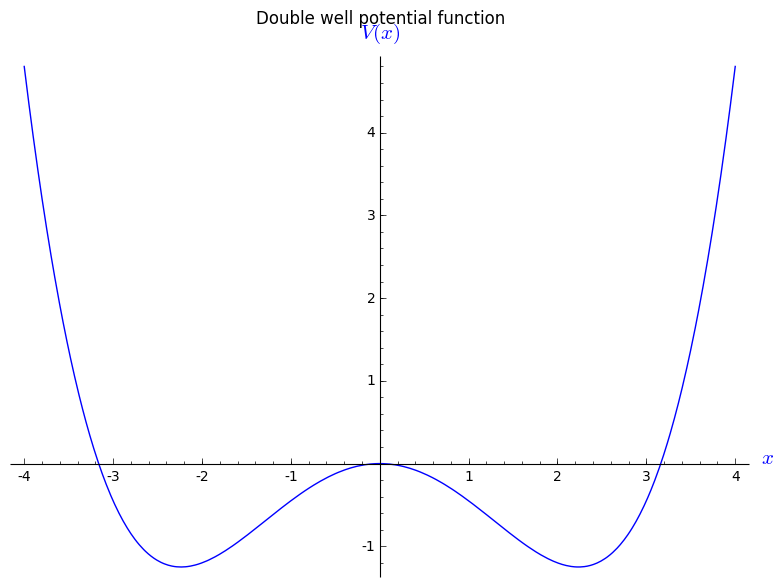
\includegraphics[width=0.6\textwidth]{pics/19_1.png} % INSERIRE QUI LO SCHEMA PER ISING
\caption{Schema di $f_{eff}(m)$ per Ising, $T < T_c$ (doppia buca).}
\label{fig:ch19_1}
\end{figure}

\begin{itemize}
    \item \textbf{Caso continuo (Heisenberg):} Per $T < T_c$, la situazione è diversa. Il sistema si ordina, e la magnetizzazione $\bar{m}_{eq}$ sceglie una direzione specifica nello spazio, rompendo la simmetria rotazionale continua. Tuttavia, tutte le direzioni sono equivalenti energeticamente. Il landscape dell'energia libera $f_{eff}(\bar{m})$ assomiglia a un "cappello messicano" (sombrero). C'è una valle continua di minimi degeneri che corrispondono a tutte le possibili direzioni di $\bar{m}_{eq}$ con lo stesso modulo.
\end{itemize}

\begin{figure}[h!]
\centering
% 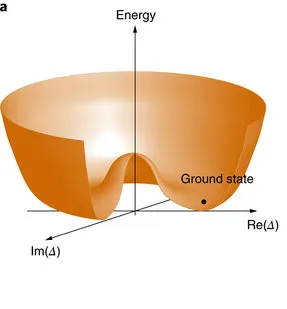
\includegraphics[width=0.6\textwidth]{pics/19_2.png} % INSERIRE QUI LO SCHEMA PER HEISENBERG
\caption{Schema di $f_{eff}(\bar{m})$ per Heisenberg (2D), $T < T_c$ (cappello messicano).}
\label{fig:ch19_9}
\end{figure}

Le fluttuazioni del modulo della magnetizzazione (salire/scendere le pareti del cappello) sono "dure" (costano energia). Tuttavia, le fluttuazioni lungo la valle dei minimi (cambiamenti nella direzione della magnetizzazione mantenendo il modulo costante) sono "soffici" e non costano energia (o costano molto poco a grandi lunghezze d'onda). Queste fluttuazioni soffici sono chiamate \textbf{modi di Goldstone} e sorgono ogni volta che una simmetria continua viene rotta spontaneamente.
La presenza di modi di Goldstone rende le fluttuazioni più importanti nei sistemi con simmetria continua.

La dimensionalità critica inferiore (la dimensione al di sotto della quale non c'è ordine per $T>0$) può essere più alta. Ad esempio, il modello di Ising ordina per $d \ge 2$, mentre il modello di Heisenberg ordina per $d \ge 3$.
Per $T < T_c$ (non solo a $T_c$), nella fase ordinata, le funzioni di correlazione connesse possono decadere come leggi di potenza a causa di questi modi soffici, invece che esponenzialmente. Questo significa che trovare un decadimento a legge di potenza non implica necessariamente che il sistema sia al punto critico $T_c$; potrebbe essere in una fase a bassa temperatura con rottura di simmetria continua.


\section{Calcolo Approssimato della Funzione di Correlazione per $T \ll T_c$ (Modi di Goldstone)}
Consideriamo un modello con simmetria continua (es. Heisenberg) a temperature molto basse rispetto a $T_c$, dove il sistema è fortemente ordinato.
L'Hamiltoniana è $H = -J \sum_{ij} m_{ij} \bar{S}_i \cdot \bar{S}_j$ dove $m_{ij}=1$ per primi vicini e 0 altrimenti.
La funzione di partizione è data da:

\begin{align*}
Z &= \int d\bar{S} e^{-\beta H(s)} \quad \quad \quad \quad \quad \bar{S} = \{\bar{S}_1, \dots, \bar{S}_N\} \\ 
&= \int d\bar{S} e^{+\beta J \sum \bar{S}_i \cdot \bar{S}_j} \delta(S_i^2 - 1)
\end{align*}

In questa fase, la magnetizzazione globale $\langle \bar{S} \rangle$ punta in una certa direzione, diciamo $\hat{n}$. Ogni spin locale $\bar{S}_i$ sarà quasi allineato con $\hat{n}$, ma avrà piccole fluttuazioni trasversali $\bar{\pi}_i$. Possiamo scrivere:

\begin{equation} \label{eq:ch19_31}
\bar{S}_i = S_i^L \hat{n} + \bar{\pi}_i
\end{equation}

dove $S_i^L$ è la componente longitudinale e $\bar{\pi}_i \cdot \hat{n} = 0$. Poiché $|\bar{S}_i|^2 = 1$, abbiamo:
$(S_i^L)^2 + |\bar{\pi}_i|^2 = 1$.
Per $\pi_i = |\bar{\pi}_i| \ll 1$ (piccole fluttuazioni trasversali), possiamo approssimare la componente longitudinale:

\begin{equation} \label{eq:ch19_32}
S_i^L = \sqrt{1 - \pi_i^2} \approx 1 - \frac{\pi_i^2}{2}
\end{equation}

Sostituendo questo nell'Hamiltoniana e sviluppando $\bar{S}_i \cdot \bar{S}_j$ fino ai termini quadratici in $\pi$:

\begin{align*} 
\bar{S}_i \cdot \bar{S}_j &= S_i^L S_j^L + \bar{\pi}_i \cdot \bar{\pi}_j \\ 
&\approx \left(1-\frac{\pi_i^2}{2}\right)\left(1-\frac{\pi_j^2}{2}\right) + \bar{\pi}_i \cdot \bar{\pi}_j \\ 
&\approx 1 - \frac{\pi_i^2}{2} - \frac{\pi_j^2}{2} + \bar{\pi}_i \cdot \bar{\pi}_j 
\end{align*}

L'Hamiltoniana (ignorando i termini costanti) diventa un'Hamiltoniana quadratica per i campi $\bar{\pi}_i$, che rappresentano le fluttuazioni trasversali (modi di Goldstone).

\begin{equation} \label{eq:ch19_33}
H \approx \text{const} + J \sum_{ij} m_{ij} \left( -\pi_i^2 + \bar{\pi}_i \cdot \bar{\pi}_j \right)
\end{equation}

(considerando la simmetria di $m_{ij}$ e che i termini $\sum \pi_i^2$ e $\sum \pi_j^2$ danno lo stesso contributo).
Questa può essere riscritta usando l'operatore Laplaciano discreto $\Lambda_{ij}$:

\begin{equation} \label{eq:ch19_34}
H \approx \sum_{ij} \Lambda_{ij} \bar{\pi}_i \cdot \bar{\pi}_j
\end{equation}

Con:
\begin{equation} \label{eq:ch19_35}
\Lambda_{ij} = -m_{ij} + \delta_{ij} \sum_k m_{ik} 
\end{equation}

Nel limite continuo: $\Lambda_{ij} \rightarrow -L^2 \nabla^2$.
La probabilità di una configurazione $\{\bar{\pi}_i\}$ è data da:

\begin{equation} \label{eq:ch19_36}
P(\{\bar{\pi}_i\}) = \frac{1}{Z} e^{-\beta J \sum \Lambda_{ij} \bar{\pi}_i \cdot \bar{\pi}_j} \; \delta\left(\sum_i \bar{\pi}_i\right)
\end{equation}

dove la $\delta$ rappresenta il vincolo che la somma delle fluttuazioni trasversali non alteri la magnetizzazione globale, $\sum_i \bar{\pi}_i = 0$.
Nello spazio di Fourier, si trova:

\begin{equation} \label{eq:ch19_37}
C^c(\bar{q}) = \frac{1}{Z} \int d\hat{\pi}(\bar{q}) \hat{\pi}(\bar{q}) \hat{\pi}(-\bar{q}) e^{-\beta \sum q^2 |\hat{\pi}(\bar{q})|^2} \delta(\hat{\pi}(0))
\end{equation}

Essendo l'Hamiltoniana Gaussiana, il calcolo della funzione di correlazione per questi modi è standard. La funzione di correlazione per i modi di Goldstone nello spazio di Fourier risulta essere:

\begin{equation} \label{eq:ch19_38}
C^c(\bar{q}) \sim \frac{1}{q^2} \quad (\text{per } q \neq 0)
\end{equation}

Antitrasformando questa espressione per ottenere la funzione di correlazione nello spazio reale, si ottiene:

\begin{equation} \label{eq:ch19_39}
C^c(\bar{r}_{ij}) = \int d\bar{\pi}_i \delta\left(\sum_k \bar{\pi}_k\right) e^{-\beta J \sum_{kl} \Lambda_{kl} \bar{\pi}_k \cdot \bar{\pi}_l} (\bar{\pi}_i \cdot \bar{\pi}_j)
\end{equation}

È un decadimento a legge di potenza. In $d$ dimensioni:

\vspace{0.5cm}
\noindent\fbox{%
    \parbox{\dimexpr\linewidth-2\fboxsep-2\fboxrule\relax}{%
        \begin{equation} \label{eq:ch19_40}
        C^c(r) \sim \frac{1}{r^{d-2}}
        \end{equation}
    }%
}
\vspace{0.5cm}

Per $d=3$, questo dà $C^c(r) \sim \frac{1}{r}$.
Questo dimostra come i modi di Goldstone, presenti nella fase ordinata ($T < T_c$) di un sistema con simmetria continua rotta spontaneamente, portino a correlazioni a lungo raggio (decadimento a legge di potenza) anche lontano dal punto critico $T_c$. Le fluttuazioni $\bar{\pi}_i$ sono direttamente collegate a piccole rotazioni della magnetizzazione globale, e quindi rappresentano i modi di Goldstone.
